\documentclass[a4paper, 12pt]{scrartcl}
\usepackage{amsfonts}
\usepackage[a4paper]{geometry}
\usepackage{alltt}
\usepackage{lmodern}
\usepackage{amssymb}
\usepackage{mathtools}
\usepackage{amsmath}
\usepackage{enumerate}
\usepackage{float}
\usepackage{graphicx}
\usepackage{hyperref}
\usepackage{array}
\usepackage{listings}
\usepackage{fullpage}
\usepackage[parfill]{parskip}
\usepackage[utf8]{inputenc}
\usepackage[english]{babel}

\graphicspath{ {images/} }

\title{Space Rave Documentation}
\subtitle{Interactive Visual Computing WiSe 14/15}
\author{Arne Beer, MN 6489196\\
        Rafael Epplee, MN 6269560\\
        Sven-Hendrik Haase, MN 6341873}

\begin{document}
\maketitle \section{Introduction}

    \begin{figure}[H]
        \centering
        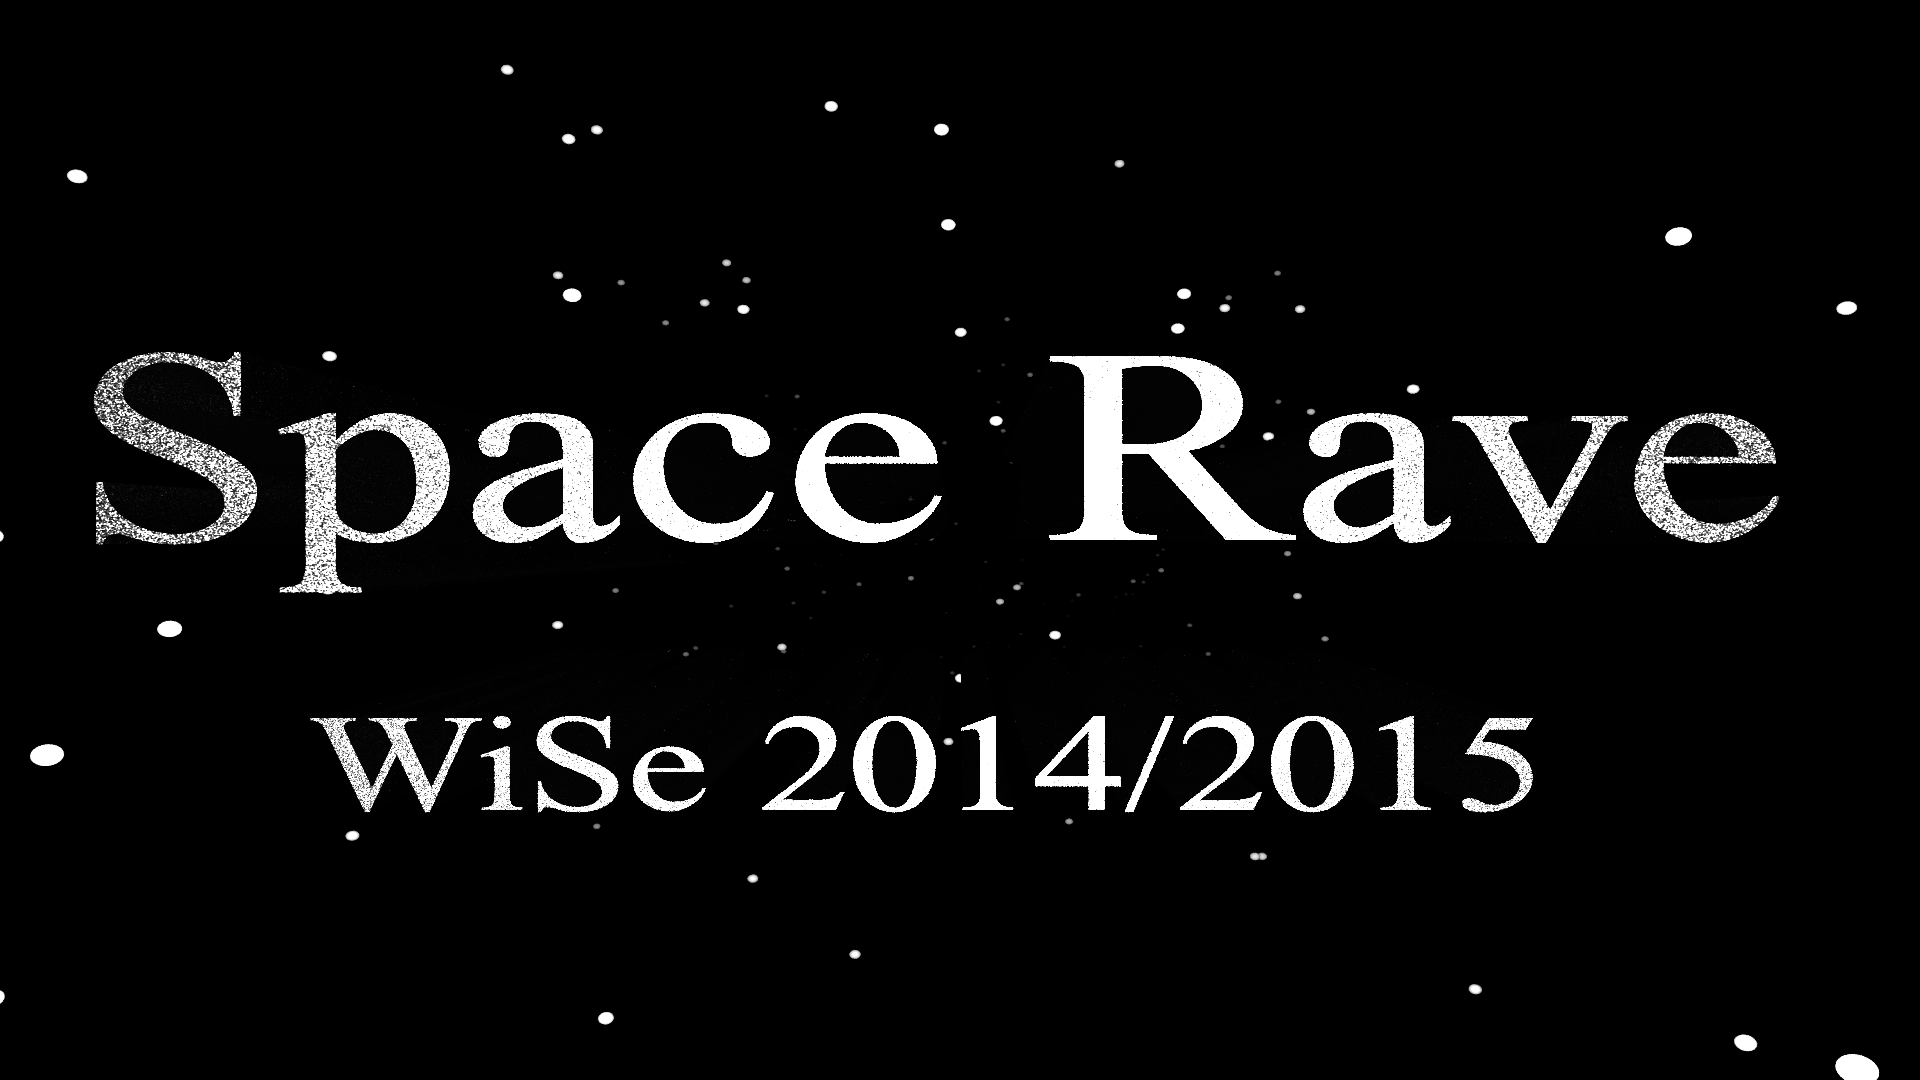
\includegraphics[scale=0.23]{render_title}
        \caption{Title scene}
        \label{fig:title}
    \end{figure}

    For our IVC project ``Space Rave'', we set out to explore the emotional impact of a music video
    that is synchronized to the contemporary electronic dance music song ``Strobe'' by Deadmau5. We
    chose this song due to its regular profile and agreeable electronic character.  The video
    consists of three distinct scenes while the visuals are set to up to represent an abstract
    spacescape throughout the scenes. The visuals consist of procedurally generated stars which
    pulse rythmically and swiftly with every kick, a procedural, fluctuating background nebula and
    a tastefully hand-modelled spaceship.

    \begin{figure}[H]
        \centering
        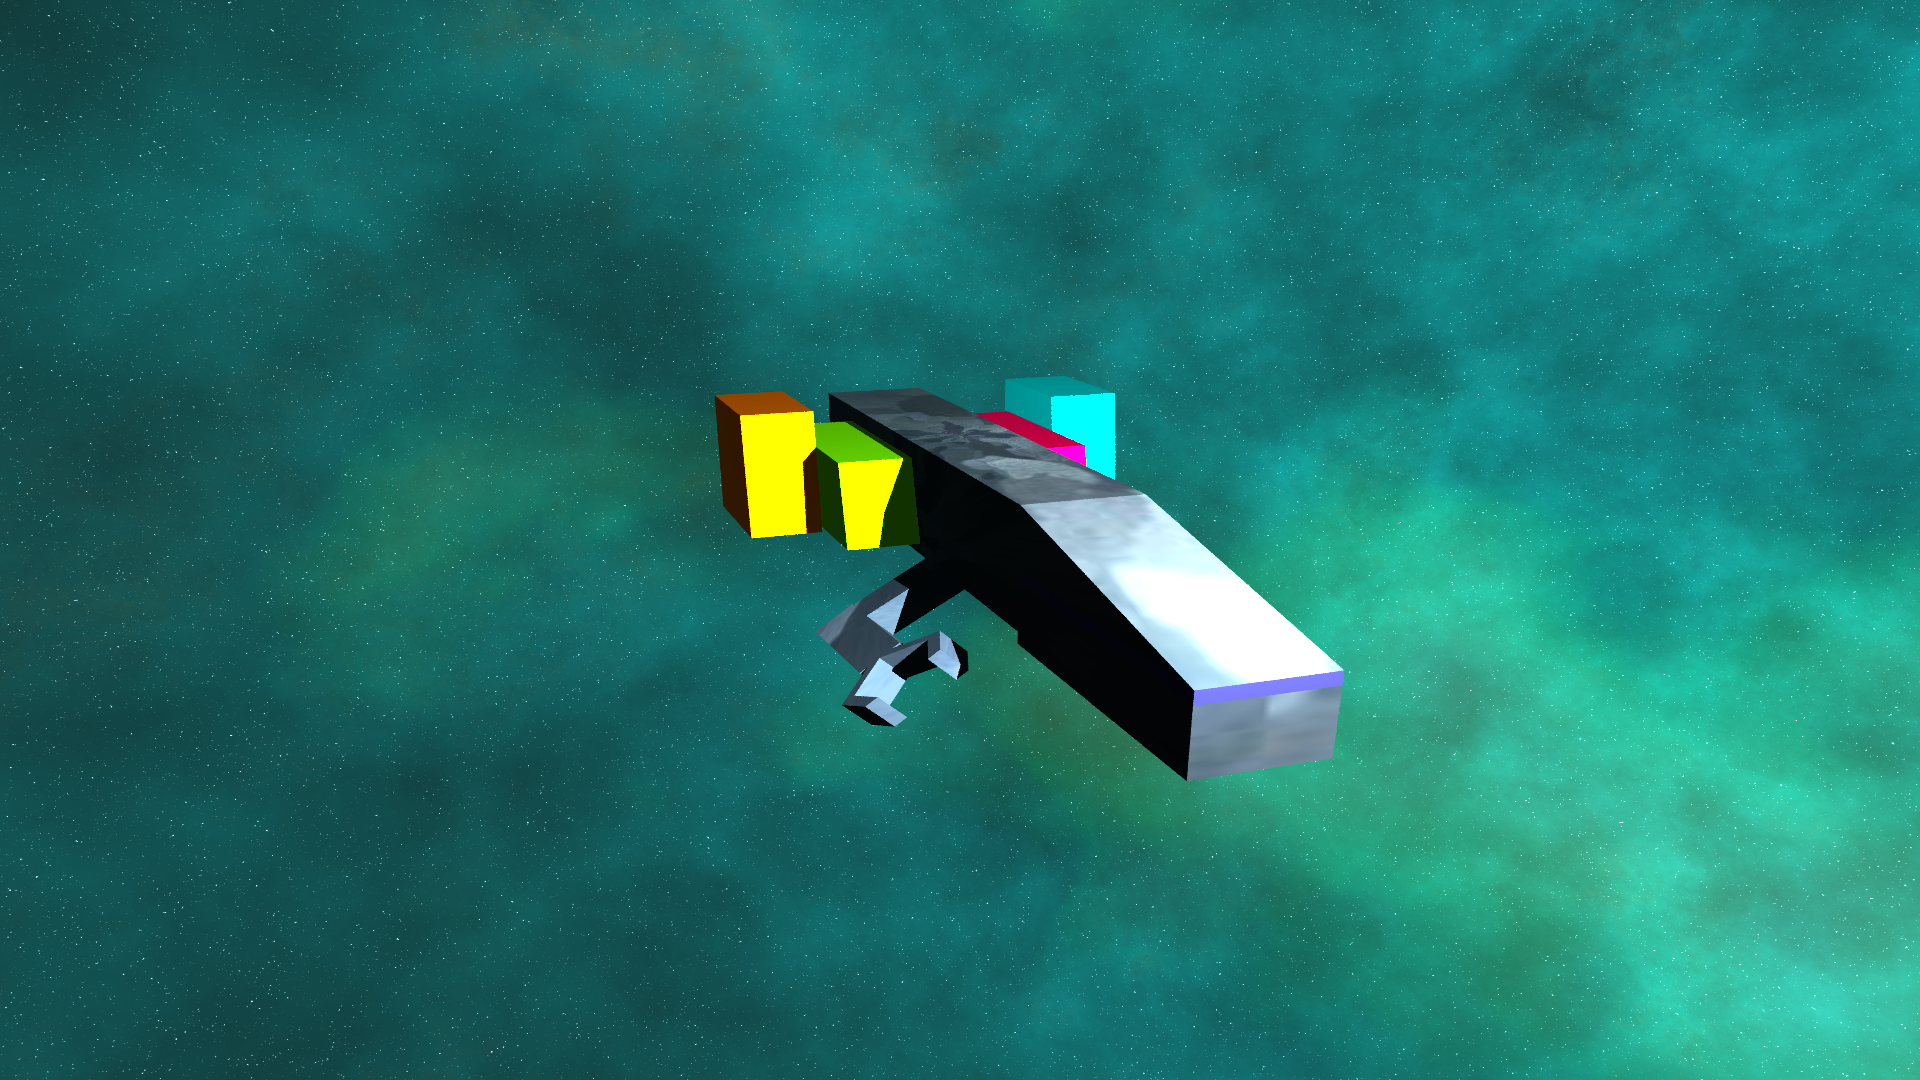
\includegraphics[scale=0.23]{render_breakdown}
        \caption{Breakdown scene}
        \label{fig:breakdown}
    \end{figure}

    From a technical standpoint, we used POV-Ray to generated the images and Audacity to analyze
    the music to find beats and chords. The timings were particuarly hard to get right.

    It should be noted that while we do not own the rights to the song we used, we believe that we
    are using this song in good faith in our transformative work under Fair Use.

    \begin{figure}[H]
        \centering
        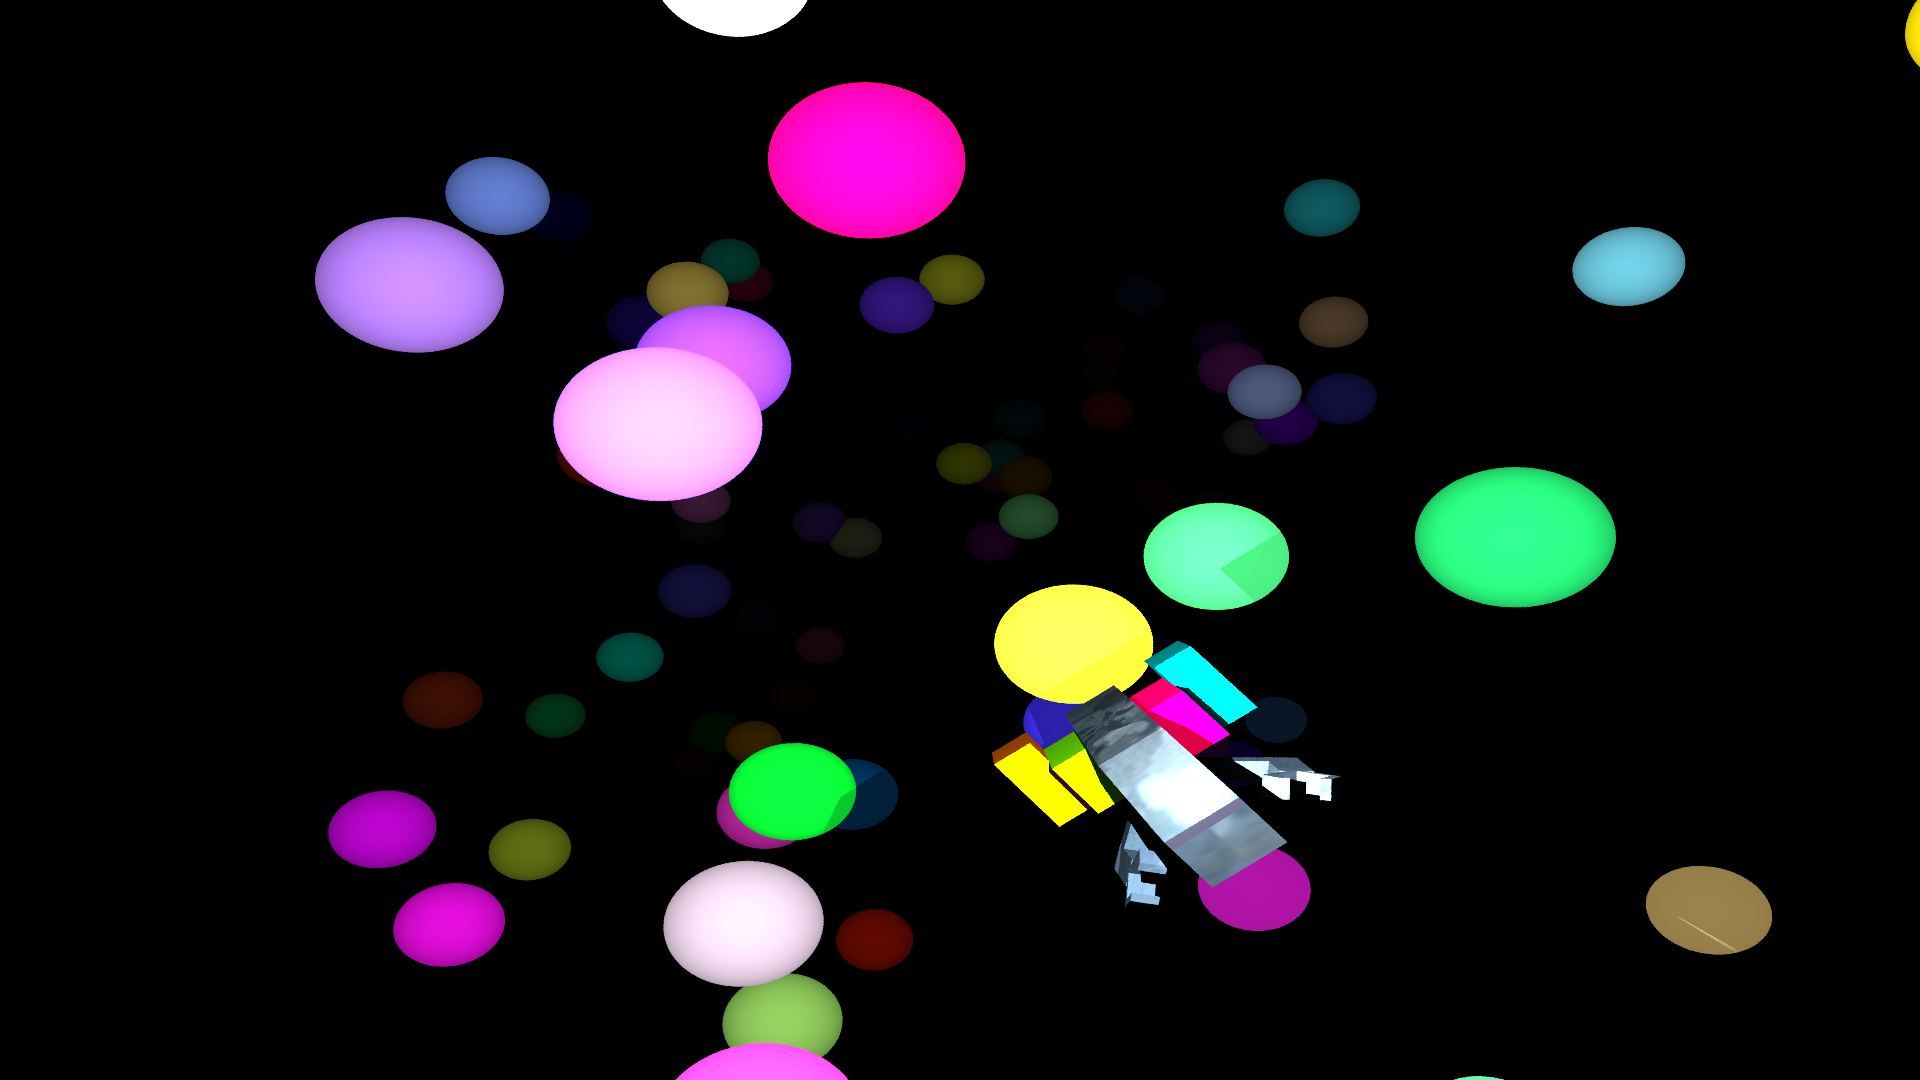
\includegraphics[scale=0.23]{render_part2}
        \caption{Second part scene}
        \label{fig:part2}
    \end{figure}

    \section{Extracting rythm information from the sound file}

    Since POV-Ray does come with any kind of Fourier transformation, we had to analyze the song by
    hand with Audacity (see~\ref{fig:main}). While this worked fairly well, we had to be very
    careful about the sub-second timings which are easy to offset by a few milliseconds which ruins
    the whole experience. For beat extraction, we used Audacity's helpful beat finder tool (see~\ref{fig:beat}) which resulted in Audacity giving us annotations where the beats were located.

    In order to find the chords, we used the spectrogram view (see~\ref{fig:spectrogram}) which
    allowed us to visually find the correct positions.

    \begin{figure}[H]
        \centering
        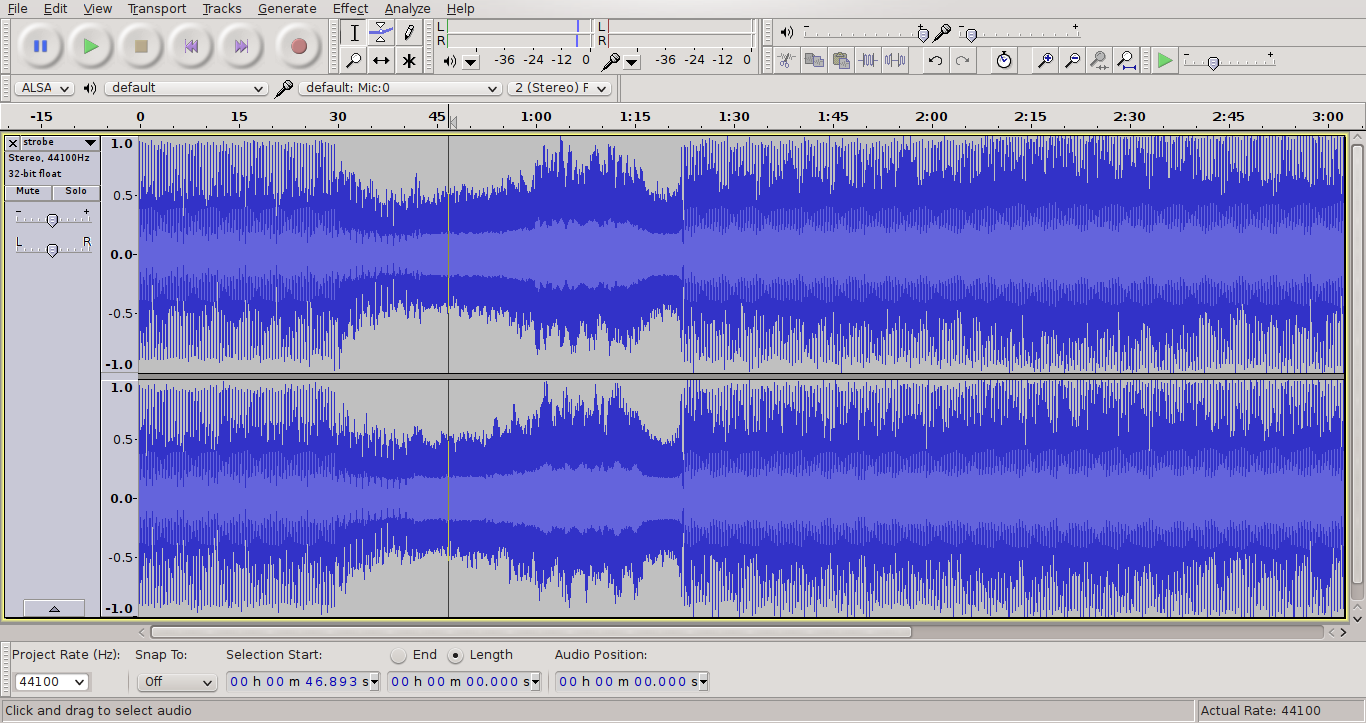
\includegraphics[scale=0.4]{audacity_main}
        \caption{Audacity main view of the track}
        \label{fig:main}
    \end{figure}

    \begin{figure}[H]
        \centering
        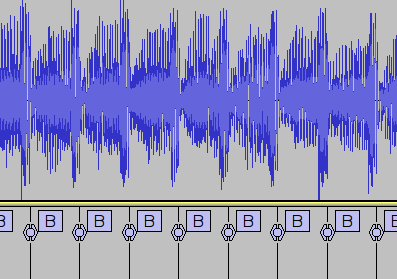
\includegraphics{audacity_beat}
        \caption{Beat analysis using Audacity's beat finder}
        \label{fig:beat}
    \end{figure}

    \begin{figure}[H]
        \centering
        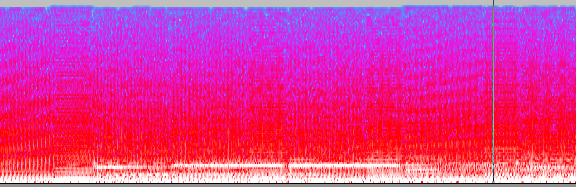
\includegraphics{audacity_spectrum}
        \caption{Spectrogram view}
        \label{fig:spectrogram}
    \end{figure}

    \section{Scenes}
    \subsection{Intro}

    The intro is composed by creating a starfield and moving the titles towards the camera.
    The starfield is generated by adding spheres with a random position and scaling their size
    depending on the beat.

    The title is a simple union of text objects using timrom.ttf with a length of 5. To make
    it look more interesting we applied a Polished\_Chrome texture with some bumps and a little
    reflection for a shiny look. The camera is constantly moving forward, while the titles are
    slowly moving towards the camera. All stars got a static position and aren't moving at all.

    \subsection{Breakdown}

    Lorem ipsum dolor sit amet, consetetur sadipscing elitr, sed diam nonumy eirmod
    tempor invidunt ut labore et dolore magna aliquyam erat, sed diam voluptua. At
    vero eos et accusam et justo duo dolores et ea rebum. Stet clita kasd gubergren,
    no sea takimata sanctus est Lorem ipsum dolor sit amet.

    \subsection{Part Two}

    Lorem ipsum dolor sit amet, consetetur sadipscing elitr, sed diam nonumy eirmod
    tempor invidunt ut labore et dolore magna aliquyam erat, sed diam voluptua. At
    vero eos et accusam et justo duo dolores et ea rebum. Stet clita kasd gubergren,
    no sea takimata sanctus est Lorem ipsum dolor sit amet.

    \section{Creating the Starfield}

    \section{Modeling the Spaceship}

    We didn't use any modeling tool for making the spaceship. Instead, we opted for a blocky, ``minecrafty'' style with almost no details. We used unions to combine mostly boxes and prisms into quite a basic shape. Even the most complex part, the claws, are built with boxes and prisms.

    The size of the ship itself and various parts is easily customizable through local values declared at the top of \texttt{ship.inc}.

    Most parts of the ship are actually mirror-symmetric, like the base body, the claws and the window in the front. To minimize effort, we just modeled those parts in half and then mirrored them using duplication and scaling.

    The only non-symmetric parts of the ship are the engines at the rear end. They are each modeled on their own, each having a distinctive color.

    \section{Timing animations according to the song}

    In order to get accurate timings, we used milliseconds with POV-Ray. Since POV-Ray only
    directly supports seconds, we multiplied all numbers by 1000 to get better resolution.
    The first step towards that was figuring out the exact length of the song which is
    \(3m32.067s\) which in turn is \(212.067s\). Since we wanted to use 60 FPS for fluid motion
    this resulted in \(212.067s \times 60 = 12724\) frames. 

    We then ran POV-Ray with the following settings:
    \begin{verbatim}+KFI1 +KFF12724 +KF12724.0\end{verbatim}
    This allowed us to use the \texttt clock variable with actual frames which was very convenient
    and turned out to be accurate enough for millisecond timings.

    For more convenience, we defined macros for beats and chords which would give us a float value
    of the position within a beat or chord respectively.

    The relevant section looks like this:

    \begin{verbatim}
#declare Beat1_Start = 33.96;
#declare Beat1_Period = 28.14;

#declare BGSynths_Start = 2426;
#declare BGSynths_Period = 21.18; // frames

#declare Beat2_Start = 4952;
#declare Beat2_Period = 28.14; // frames

#declare start_part1_fade = 0;
#declare end_part1_fade = 800;
#declare start_break_down_fade = 1800;
#declare end_break_down_fade = 2400;
#declare start_focus_break_down = 3000;
#declare end_focus_break_down = 3800;
#declare start_part2_fade = 4920;
#declare end_part2_fade = 4951;
#declare end_song = 12724;
#declare fade_out_start = 9462;
#declare fade_out_end = 9840;

#macro Beat1()
    mod((clock + Beat1_Start) * 10000, Beat1_Period * 10000) /
        (Beat1_Period * 10000)
#end

#macro BGSynths()
    mod((clock + BGSynths_Start) * 10000, BGSynths_Period * 10000) /
        (BGSynths_Period * 10000)
#end

#macro BGSynths_2()
    mod((clock + BGSynths_Start) * 10000, BGSynths_Period * 2 * 10000) /
        (BGSynths_Period * 2 * 10000)
#end

#macro Beat2()
    mod((clock + Beat2_Start) * 10000, Beat2_Period * 10000) /
        (Beat2_Period * 10000)
#end
    \end{verbatim}

    \section{Background Generation}

    To create a starfield and nebula we used a comination of 2 spheres and a sky\_sphere. \\ 
    The sky\_sphere got a pigment that gets a perlin noise pigment map, which consists of three different colormaps. As a result we generate the procedural starfield. \\
    In order to generate a nebula we create spheres and define the interior of those. There are two different spheres with different interior medias. \\
    The first nebula is generated by creating a hollow, transparent sphere and filling it with an interior, which is defined by a media that got 2 different densities. A density is used to vary the density of particles inside a media.
    By adding two densities we get the intersection of both densities. The first density is defined by a rampwave on a colormap, to get a nice transition for the colors. We decided to spice this up by translating, warping everything and translating it back. As a result we get a nice nebula effect. \\
    The second density simply defined by a rampwave on a colormap and different density values inside the color map.

    The other sphere is quite similar to the first one, except that it got other colors, a single density and we actually vary the turbulence of density to the beat to create a wobbly effect on the nebula. 
    We use some other values like octaves, frequency and labmda to create diffent nebula look.

    \section{Ship movement}

    The movement of the last ship in the last scene has been achieved by using a spline. We
    use a natural\_spline to create a smoother trajectory. The spline is applied by using
    Trans\_Spline with pretty high values for foresight and banking, because the ship actually
    moves at -60*z per second.

    \section{Summary}

    In conclusion, we think the project was a fun and challenging excercise. Working against the
    limitations of POV-Ray was, at times, frustrating while additionally its rendering speed was
    inferior to modern tools. Due to the very timing critical nature of our project, we had to do
    many re-renders of the same few hundred frames.

    All in all, we think we reached our goal of creating a proper visual animation to the song
    track that we chose.

\end{document}
